%==============================================================
%  MUGHAL-AUTH AI — BTP Submission Report
%  Tectonic-compatible LaTeX (compile with: tectonic main.tex)
%
%  All 5 architecture & data-flow diagrams are drawn natively
%  in vector LaTeX (TikZ) — zero external diagram files needed.
%
%  Place your UI screenshots in report/images/:
%    fig_cover_logo.png       — IIT Kharagpur seal (already included)
%    fig_ui_home.png          — Screenshot: Home page / image uploader
%    fig_ui_verdict.png       — Screenshot: Verdict banner (Mughal YES)
%    fig_ui_multihead.png     — Screenshot: Multi-head classification cards
%    fig_ui_reasoning.png     — Screenshot: Art-historian reasoning panel
%    fig_ui_features.png      — Screenshot: Visual features & motif pills
%    fig_ui_history.png       — Screenshot: History drawer open
%==============================================================

\documentclass[12pt, a4paper, twoside]{article}

%--------------------------------------------------------------
% Packages
%--------------------------------------------------------------
\usepackage[T1]{fontenc}
\usepackage[utf8]{inputenc}
\usepackage{lmodern}
\usepackage{microtype}

% Page geometry
\usepackage[
  a4paper,
  top=2.5cm, bottom=2.5cm,
  left=3.0cm, right=2.5cm,
  headheight=14pt
]{geometry}

% Colors — deep palette matching museum aesthetic
\usepackage{xcolor}
\definecolor{MughalGreen}{RGB}{27,67,50}      % deep forest green
\definecolor{ImperialGold}{RGB}{180,131,34}    % antique gold
\definecolor{ObsidianBlue}{RGB}{15,23,42}      % near-black blue
\definecolor{IvoryWhite}{RGB}{250,246,237}     % parchment
\definecolor{MutedGray}{RGB}{100,116,139}      % slate gray
\definecolor{AccentRed}{RGB}{185,28,28}        % crimson for OOD
\definecolor{SoftBlue}{RGB}{29,78,216}         % link / accent blue
\definecolor{PurpleHead}{RGB}{109,40,217}      % classifier head purple

% Typography
\usepackage{palatino}      % elegant serif body
\usepackage{setspace}
\setstretch{1.25}

% Headers & footers
\usepackage{fancyhdr}
\pagestyle{fancy}
\fancyhf{}
\fancyhead[LE,RO]{\small\textcolor{MughalGreen}{\textbf{Mughal-Auth AI}} — BTP Report, IIT Kharagpur}
\fancyhead[RE,LO]{\small\textcolor{MutedGray}{\leftmark}}
\fancyfoot[C]{\small\textcolor{MutedGray}{\thepage}}
\renewcommand{\headrulewidth}{0.4pt}
\renewcommand{\headrule}{\hbox to\headwidth{\color{MughalGreen}\leaders\hrule height \headrulewidth\hfill}}

% Section styling
\usepackage{titlesec}
\titleformat{\section}
  {\color{MughalGreen}\large\bfseries}
  {\thesection}{1em}{}[\color{MughalGreen}\titlerule]
\titleformat{\subsection}
  {\color{ObsidianBlue}\normalsize\bfseries}
  {\thesubsection}{1em}{}
\titleformat{\subsubsection}
  {\color{PurpleHead}\normalsize\itshape\bfseries}
  {\thesubsubsection}{1em}{}

% Graphics & TikZ Vector Diagrams
\usepackage{graphicx}
\usepackage{float}
\usepackage{caption}
\usepackage{tikz}
\usetikzlibrary{arrows.meta, positioning, shapes.geometric, fit, backgrounds, calc}

\captionsetup{
  font=small,
  labelfont={bf,color=MughalGreen},
  textfont={it,color=ObsidianBlue},
  labelsep=period,
  skip=6pt
}
\graphicspath{{images/}}

% Macro: render screenshot if present in images/, else clean placeholder box
\newcommand{\screenshotorplaceholder}[1]{%
  \IfFileExists{images/#1.png}{%
    \includegraphics[width=\linewidth]{#1}%
  }{%
    \fcolorbox{MughalGreen}{IvoryWhite}{%
      \parbox{0.94\linewidth}{%
        \centering\vspace{1.4cm}
        {\large\bfseries\color{MughalGreen}[ Screenshot Placeholder ]}\\[0.25cm]
        {\small\texttt{images/#1.png}}\\[0.15cm]
        {\footnotesize\color{MutedGray}Save the corresponding frontend screenshot at the path above and recompile with \texttt{tectonic main.tex}.}
        \vspace{1.4cm}
      }%
    }%
  }%
}

% Tables
\usepackage{booktabs}
\usepackage{tabularx}
\usepackage{longtable}
\usepackage{array}
\usepackage{multirow}
\usepackage{colortbl}
\newcolumntype{L}[1]{>{\raggedright\arraybackslash}p{#1}}
\newcolumntype{C}[1]{>{\centering\arraybackslash}p{#1}}
\newcolumntype{R}[1]{>{\raggedleft\arraybackslash}p{#1}}

% Math
\usepackage{amsmath}
\usepackage{amssymb}

% Code listings
\usepackage{listings}
\lstset{
  basicstyle=\ttfamily\small\color{ObsidianBlue},
  backgroundcolor=\color{IvoryWhite},
  frame=single,
  rulecolor=\color{MughalGreen},
  keywordstyle=\color{SoftBlue}\bfseries,
  commentstyle=\color{MutedGray}\itshape,
  stringstyle=\color{AccentRed},
  breaklines=true,
  captionpos=b,
  numbers=left,
  numberstyle=\tiny\color{MutedGray},
  xleftmargin=1.5em,
  framexleftmargin=1.5em,
  aboveskip=0.8em,
  belowskip=0.8em
}

% Hyperlinks
\usepackage[
  colorlinks=true,
  linkcolor=MughalGreen,
  citecolor=ImperialGold,
  urlcolor=SoftBlue,
  bookmarks=true,
  pdfauthor={Arka Ghosh; Anushesh; Snigdha Ghosh},
  pdftitle={Mughal-Auth AI: BTP Submission Report},
  pdfsubject={Computer Science Engineering, IIT Kharagpur}
]{hyperref}

% Callout boxes
\usepackage{tcolorbox}
\tcbuselibrary{skins, breakable}

\newtcolorbox{importantbox}[1][]{
  enhanced, breakable,
  colback=MughalGreen!8,
  colframe=MughalGreen,
  fonttitle=\bfseries\color{white},
  coltitle=white,
  attach boxed title to top left={yshift=-2mm, xshift=4mm},
  boxed title style={colback=MughalGreen, rounded corners},
  title=Key Insight, #1
}

\newtcolorbox{notebox}[1][]{
  enhanced, breakable,
  colback=SoftBlue!6,
  colframe=SoftBlue,
  fonttitle=\bfseries\color{white},
  coltitle=white,
  attach boxed title to top left={yshift=-2mm, xshift=4mm},
  boxed title style={colback=SoftBlue, rounded corners},
  title=Technical Note, #1
}

\newtcolorbox{warningbox}[1][]{
  enhanced, breakable,
  colback=AccentRed!6,
  colframe=AccentRed,
  fonttitle=\bfseries\color{white},
  coltitle=white,
  attach boxed title to top left={yshift=-2mm, xshift=4mm},
  boxed title style={colback=AccentRed, rounded corners},
  title=Fail-Loud Guarantee, #1
}

% Misc
\usepackage{enumitem}
\setlist[itemize]{leftmargin=1.5em, itemsep=2pt, topsep=4pt}
\setlist[enumerate]{leftmargin=1.5em, itemsep=2pt, topsep=4pt}
\usepackage{parskip}
\usepackage{tocbibind}
\usepackage{url}
\urlstyle{same}

%==============================================================
% DOCUMENT
%==============================================================
\begin{document}

%--------------------------------------------------------------
% TITLE PAGE
%--------------------------------------------------------------
\begin{titlepage}
  \centering
  \vspace*{0.5cm}

  % Institute logo
  
\includegraphics[width=3.2cm]{fig_cover_logo}\\[0.6cm]

  {\Large\bfseries\color{MughalGreen}
    INDIAN INSTITUTE OF TECHNOLOGY KHARAGPUR}\\[0.2cm]
  {\normalsize\color{MutedGray}
    Department of Computer Science and Engineering}\\[1.2cm]

  \hrule height 1.5pt
  \vspace{0.4cm}

  {\huge\bfseries\color{ObsidianBlue}
    Mughal-Auth AI}\\[0.3cm]
  {\Large\itshape\color{ImperialGold}
    A Multi-Head Vision Transformer, Dual-Branch Feature Fusion,\\
    and Multimodal VLM Platform for\\
    Indian Miniature Painting Authentication}\\[0.4cm]

  \hrule height 1.5pt
  \vspace{0.9cm}

  {\normalsize\color{MutedGray} Report submitted in partial fulfilment of the requirements\\
  for the award of the degree of}\\[0.3cm]
  {\normalsize\bfseries Bachelor of Technology in Computer Science and Engineering}\\[1.0cm]

  {\normalsize\color{MutedGray} Submitted by}\\[0.4cm]
  \begin{tabular}{lc}
    \toprule
    \textbf{Name} & \textbf{Roll Number}\\
    \midrule
    Arka Ghosh    & 21CS10009\\
    Anushesh      & [Roll Number]\\
    Snigdha Ghosh & [Roll Number]\\
    \bottomrule
  \end{tabular}\\[1.0cm]

  {\normalsize\color{MutedGray} Under the guidance of}\\[0.3cm]
  {\normalsize\bfseries Prof.\ Partha Pratim Chakrabarti}\\
  {\normalsize\bfseries Prof.\ Partha Pratim Das}\\[1.0cm]

  \vfill
  {\normalsize\bfseries\color{MughalGreen} November 2026}
\end{titlepage}

%--------------------------------------------------------------
% FRONT MATTER
%--------------------------------------------------------------
\pagenumbering{roman}
\setcounter{page}{1}

%--- Abstract
\clearpage
\section*{Abstract}
\addcontentsline{toc}{section}{Abstract}
\markboth{Abstract}{}

\textbf{Mughal-Auth AI} is a full-stack computational connoisseurship platform that authenticates Indian miniature paintings through a hierarchical inference pipeline combining frozen Vision Transformer embeddings, 96-dimensional handcrafted art-historical descriptors, open-vocabulary iconographic motif detection, temperature-calibrated multi-head neural classification, and grounded multimodal visual language model reasoning.

The system addresses three intertwined challenges. First, the \emph{out-of-distribution problem}: closed-set softmax classifiers must not be allowed to report Mughal provenance for a modern photograph or a digitized European engraving. An embedding-space cosine-similarity gate using the top-$k$ nearest training paintings intercepts all non-miniature inputs before any classification head is activated. Second, the \emph{representation challenge}: mineral pigment chemistry, \textit{nim-qalam} stippled brushwork, and manuscript iconography lie beyond the discriminative reach of a plain ImageNet-pretrained feature extractor. A dual-branch fusion pipeline concatenates frozen ViT-B/16 global and region-pooled embeddings (768-d each) with four categories of handcrafted descriptors (colour, texture, stroke, layout — 96-d total) into a 1,632-dimensional unified vector. Third, the \emph{calibration challenge}: raw neural logits overstate certainty on borderline paintings. Post-hoc per-head Temperature Scaling aligns calibrated softmax probabilities with empirical validation-set precision.

The resulting ML engine is surfaced to end users through a full-stack web platform: a React~19/Vite~8/Tailwind CSS~v4 single-page application, an Express.js REST API server, a Node.js-to-Python child-process ML bridge, and a dual-persistence data layer. Expert curators may issue corrections through a human-in-the-loop feedback interface that feeds directly into the active retraining pipeline.

Evaluated on an 84-painting held-out test set partitioned across 65 disjoint manuscript groups, the system achieves 90.5\% accuracy and Macro F1\,=\,0.485 for Artistic School classification, 66.1\% accuracy and Macro F1\,=\,0.462 for Historical Period attribution, and passes all 169 known miniature paintings through the OOD gate while rejecting all 12 control non-miniature images.

\textbf{Keywords:} Vision Transformer, feature fusion, temperature scaling, YOLO-World, multimodal reasoning, Mughal miniature, out-of-distribution detection, full-stack deployment.

%--- Certificate
\clearpage
\section*{Certificate}
\addcontentsline{toc}{section}{Certificate}
\markboth{Certificate}{}

This is to certify that the work contained in this report, titled \textit{``Mughal-Auth AI: A Multi-Head Vision Transformer, Dual-Branch Feature Fusion, and Multimodal VLM Platform for Indian Miniature Painting Authentication''}, submitted by Arka Ghosh (21CS10009), Anushesh ([Roll Number]), and Snigdha Ghosh ([Roll Number]) to the Department of Computer Science and Engineering, Indian Institute of Technology Kharagpur, for the partial fulfilment of the requirements for the award of the degree of Bachelor of Technology in Computer Science and Engineering, is a bona fide record of the work carried out by them under my/our supervision.

\vspace{2cm}
\noindent
\begin{tabular}{p{6cm} p{6cm}}
  \underline{\hspace{5.5cm}} & \underline{\hspace{5.5cm}}\\
  Prof.\ Partha Pratim Chakrabarti & Prof.\ Partha Pratim Das\\
  Department of CSE & Department of CSE\\
  IIT Kharagpur & IIT Kharagpur\\
\end{tabular}

\vspace{1.5cm}
\noindent
\textbf{Date:} November 2026

%--- Acknowledgements
\clearpage
\section*{Acknowledgements}
\addcontentsline{toc}{section}{Acknowledgements}
\markboth{Acknowledgements}{}

The authors express their gratitude to Prof.\ Partha Pratim Chakrabarti and Prof.\ Partha Pratim Das for their guidance and encouragement throughout this project. The authors also acknowledge the museum collections and digital archives whose published catalogues formed the foundational dataset for this work. Computational resources were accessed through the institute's high-performance computing infrastructure.

%--- TOC
\clearpage
\tableofcontents

\clearpage
\listoffigures

\clearpage
\listoftables

%--------------------------------------------------------------
% MAIN MATTER
%--------------------------------------------------------------
\clearpage
\pagenumbering{arabic}
\setcounter{page}{1}

%==============================================================
\section{Introduction}
\label{sec:intro}
%==============================================================

\subsection{Motivation and Problem Statement}

The authentication of Indian miniature paintings is among the most demanding problems in computational art history. Scholars distinguish Imperial Mughal atelier works from Rajasthani and Pahari school productions through a layered analysis of pigment chemistry, brushwork morphology, iconographic conventions derived from Sanskrit textual traditions, and manuscript provenance recorded in Persian administrative registers. This domain knowledge is concentrated in a small number of specialist curators at auction houses and museum conservation departments, creating a severe bottleneck for the growing volume of historical works entering the global art market.

Computational approaches to miniature classification face three obstacles that generic image classification systems cannot resolve:

\begin{enumerate}
  \item \textbf{Out-of-distribution inputs.} Closed-set classifiers assign probabilities summing to 100\% across known labels regardless of whether the input is a miniature painting, a modern photograph, or a digitized document. Without an explicit guard, any photograph submitted to such a system receives a spurious Mughal attribution.
  \item \textbf{Representational inadequacy.} Standard ImageNet-pretrained features capture object identity but not pigment formulation, \textit{wasli} paper fibre texture, or iconographic ensemble composition—the signals that actually distinguish Mughal from Rajasthani production.
  \item \textbf{Overconfident probabilities.} Raw neural logits from trained classifiers systematically overstate certainty, particularly on atypical or borderline examples. A connoisseur who is 85\% certain reports that uncertainty; an uncalibrated classifier reporting 99\% certainty on the same painting provides misleading information to the expert evaluating the system's output.
\end{enumerate}

\subsection{Contributions}

This report documents a multi-layer system that addresses all three obstacles, implemented as a production-ready web platform. The contributions span three dimensions:

\begin{itemize}
  \item \textbf{Machine Learning Pipeline.} Manuscript-grouped leak-free data partitioning; ViT-B/16 and CLIP dual OOD gate; dual-branch 1,632-d feature fusion; four-head neural classifier with balanced multi-task loss; per-head Temperature Scaling calibration; YOLO-World open-vocabulary motif detection; Qwen~2.5-VL multimodal cross-check.
  \item \textbf{Full-Stack Engineering.} React 19/Vite/Tailwind CSS~v4 single-page application with eleven purpose-built components; Express.js REST API server; Node.js-to-Python child-process ML bridge; dual-persistence data layer (MongoDB + JSON fallback); Vercel frontend deployment; Hugging Face Spaces GPU backend.
  \item \textbf{Human-in-the-Loop Feedback System.} Expert Review Modal connected to a feedback API that persists curator corrections and enables active retraining.
\end{itemize}

\subsection{Report Organisation}

Section~\ref{sec:related} briefly situates this work in the literature. Section~\ref{sec:data} describes the dataset and leak-free splitting strategy. Section~\ref{sec:ml} covers the complete ML inference pipeline in seven stages. Section~\ref{sec:backend} details the backend architecture and ML bridge. Section~\ref{sec:frontend} covers the frontend design and all UI components. Section~\ref{sec:integration} describes the end-to-end data flow. Section~\ref{sec:results} reports quantitative benchmark results. Section~\ref{sec:conclusion} concludes.

%==============================================================
\section{Related Work}
\label{sec:related}
%==============================================================

\subsection{Vision Transformers for Cultural Heritage}

The Vision Transformer (ViT)~\cite{dosovitskiy2021image} has demonstrated superior transfer capability on fine-grained recognition tasks where convolutional networks struggle. Applications to cultural heritage have included painting style transfer~\cite{gatys2016neural}, period classification~\cite{tan2016ceci}, and artist attribution from brushwork statistics. The frozen ViT-B/16 backbone employed here provides an ${\ell_2}$-normalised 768-dimensional embedding space that is remarkably separable across art historical schools without domain-specific fine-tuning.

\subsection{Out-of-Distribution Detection}

Distributional shift detection methods include maximum softmax probability~\cite{hendrycks2017baseline}, energy scoring~\cite{liu2020energy}, Mahalanobis distance in feature space~\cite{lee2018mahalanobis}, and embedding-space nearest-neighbour methods~\cite{sun2022knn}. The cosine nearest-neighbour gate adopted here is a computationally lightweight variant of the latter, requiring only a single matrix multiply against the precomputed training corpus embeddings at inference time.

\subsection{Model Calibration}

Guo et al.~\cite{guo2017calibration} demonstrated that modern deep networks are poorly calibrated, with Reliability Diagrams showing systematic overconfidence. Post-hoc Temperature Scaling—dividing all logits by a learned scalar temperature before softmax—is the simplest and most effective calibration method for single-class heads. The multi-head variant used here fits one temperature per classification head on the 85-painting validation set.

\subsection{Open-Vocabulary Object Detection}

YOLO-World~\cite{cheng2024yoloworld} extends the YOLO detection framework with a CLIP text encoder, enabling zero-shot detection of arbitrary text-specified categories without bounding-box training annotations. This property is essential for miniature iconography, where domain-specific Sanskrit terms (\textit{nayika}, \textit{kadamba}, \textit{bhramara}) have zero coverage in CLIP's training corpus but their plain-language English translations (\textit{woman}, \textit{tree}, \textit{bee}) are well-represented.

%==============================================================
\section{Dataset and Partitioning}
\label{sec:data}
%==============================================================

\subsection{Corpus Characteristics}

The curated corpus comprises 564 paintings drawn from digitised museum collections and published catalogues, spanning three primary schools (Mughal, Rajasthani, Pahari), six imperial periods (Akbar, Jahangir, Shah Jahan, Aurangzeb, Classical Mughal, Late Mughal / 18th Century), 35 Ragamala musical modes, and sparse artist attribution data.

A critical structural property of historical miniature datasets is \emph{manuscript cohesion}: multiple folios from a single royal album (e.g., the Tuti-nama commission of Akbar's court, $n = 153$ folios) share border patterns, \textit{wasli} paper aging, and pigment recipes. Standard random splitting leaks these shared signals across train and test sets, artificially inflating reported accuracy.

\subsection{Manuscript-Grouped Leak-Free Splitting}

To prevent leakage, all 564 paintings are grouped into 341 disjoint manuscript or album identifiers. A multi-objective stratified optimisation procedure (10,000 random trials minimising absolute size deviation subject to per-category, per-school, and per-period representation constraints) partitions these groups into three non-overlapping splits:

\begin{table}[H]
  \centering
  \caption{Manuscript-grouped data partitions with zero group overlap.}
  \label{tab:splits}
  \rowcolors{2}{IvoryWhite}{white}
  \begin{tabularx}{\linewidth}{L{2.4cm} C{1.5cm} C{1.4cm} C{2.0cm} C{1.4cm} L{3.5cm}}
    \toprule
    \rowcolor{MughalGreen!15}
    \textbf{Split} & \textbf{Paintings} & \textbf{Share} & \textbf{Groups} & \textbf{Overlap} & \textbf{Role}\\
    \midrule
    Train     & 395 & 70.0\% & 216 & 0\% & Weight training, feature standardisation\\
    Validation & 85 & 15.1\% & 60  & 0\% & Early stopping, Temperature Scaling fit\\
    Test      & 84  & 14.9\% & 65  & 0\% & Held-out benchmark evaluation\\
    \midrule
    \textbf{Total} & \textbf{564} & \textbf{100\%} & \textbf{341} & \textbf{0\%} & 395 Mughal · 134 Crops · 35 Ragamalas\\
    \bottomrule
  \end{tabularx}
\end{table}

\subsection{Label Normalisation}

Because museum metadata exhibits severe class imbalance ($\sim$90\% Mughal, $\sim$90\% Non-Ragamala), labels are normalised before training:

\begin{itemize}
  \item \textbf{School}: Three classes (\texttt{Mughal}, \texttt{Rajasthani}, \texttt{Pahari}); unseen regional classes are isolated during evaluation.
  \item \textbf{Period}: Six imperial epochs; undated paintings ($\sim$30\%) map to \texttt{IGNORE\_INDEX = -100}, exempting them from gradient contributions.
  \item \textbf{Raga}: \texttt{None} maps to \texttt{Non-Ragamala}; ultra-rare ragas ($<3$ paintings) are grouped into \texttt{Ragamala (Unspecified)}.
  \item \textbf{Artist}: Retained as a fourth head, flagged as statistically insufficient (only four attributed training paintings, all Ustad Mansur).
\end{itemize}

%==============================================================
\section{Machine Learning Inference Pipeline}
\label{sec:ml}
%==============================================================

The inference pipeline follows seven deterministic stages applied sequentially to every submitted image. No stage is skipped or bypassed; failure at any stage returns a structured error payload.

\begin{figure}[H]
  \centering
  \resizebox{\linewidth}{!}{%
  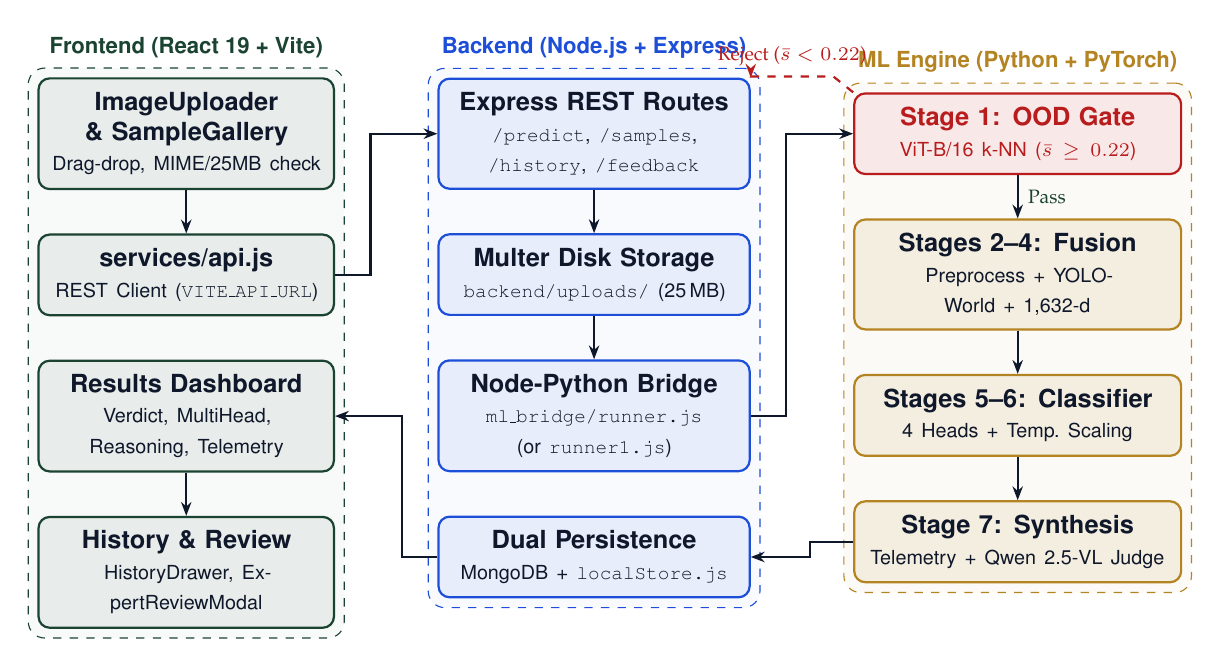
\begin{tikzpicture}[
    node distance=0.8cm and 0.9cm,
    font=\sffamily\small,
    box/.style={draw, rounded corners=4pt, align=center, minimum height=0.85cm, inner sep=5pt, line width=0.8pt},
    fe/.style={box, fill=MughalGreen!10, draw=MughalGreen, text=ObsidianBlue},
    be/.style={box, fill=SoftBlue!10, draw=SoftBlue, text=ObsidianBlue},
    ml/.style={box, fill=ImperialGold!14, draw=ImperialGold, text=ObsidianBlue},
    ood/.style={box, fill=AccentRed!10, draw=AccentRed, text=AccentRed},
    arr/.style={-{Stealth[length=5pt]}, thick, color=ObsidianBlue}
  ]
    % Frontend Tier
    \node[fe, text width=3.4cm] (ui) {\textbf{ImageUploader \& SampleGallery}\\{\scriptsize Drag-drop, MIME/25MB check}};
    \node[fe, below=0.55cm of ui, text width=3.4cm] (api) {\textbf{services/api.js}\\{\scriptsize REST Client (\texttt{VITE\_API\_URL})}};
    \node[fe, below=0.55cm of api, text width=3.4cm] (views) {\textbf{Results Dashboard}\\{\scriptsize Verdict, MultiHead, Reasoning, Telemetry}};
    \node[fe, below=0.55cm of views, text width=3.4cm] (hist) {\textbf{History \& Review}\\{\scriptsize HistoryDrawer, ExpertReviewModal}};

    % Backend Tier
    \node[be, right=1.3cm of ui, text width=3.6cm] (routes) {\textbf{Express REST Routes}\\{\scriptsize \texttt{/predict}, \texttt{/samples}, \texttt{/history}, \texttt{/feedback}}};
    \node[be, below=0.55cm of routes, text width=3.6cm] (multer) {\textbf{Multer Disk Storage}\\{\scriptsize \texttt{backend/uploads/} (25\,MB)}};
    \node[be, below=0.55cm of multer, text width=3.6cm] (bridge) {\textbf{Node-Python Bridge}\\{\scriptsize \texttt{ml\_bridge/runner.js} (or \texttt{runner1.js})}};
    \node[be, below=0.55cm of bridge, text width=3.6cm] (store) {\textbf{Dual Persistence}\\{\scriptsize MongoDB + \texttt{localStore.js}}};

    % ML Tier
    \node[ood, right=1.3cm of routes, text width=3.8cm] (ood) {\textbf{Stage 1: OOD Gate}\\{\scriptsize ViT-B/16 k-NN ($\bar{s} \ge 0.22$)}};
    \node[ml, below=0.55cm of ood, text width=3.8cm] (fusion) {\textbf{Stages 2--4: Fusion}\\{\scriptsize Preprocess + YOLO-World + 1,632-d}};
    \node[ml, below=0.55cm of fusion, text width=3.8cm] (heads) {\textbf{Stages 5--6: Classifier}\\{\scriptsize 4 Heads + Temp.\ Scaling}};
    \node[ml, below=0.55cm of heads, text width=3.8cm] (vlm) {\textbf{Stage 7: Synthesis}\\{\scriptsize Telemetry + Qwen 2.5-VL Judge}};

    % Group backgrounds
    \begin{scope}[on background layer]
      \node[draw=MughalGreen, dashed, rounded corners=6pt, fill=MughalGreen!3, fit=(ui)(api)(views)(hist), label={[font=\sffamily\bfseries\footnotesize, color=MughalGreen]above:Frontend (React 19 + Vite)}] {};
      \node[draw=SoftBlue, dashed, rounded corners=6pt, fill=SoftBlue!3, fit=(routes)(multer)(bridge)(store), label={[font=\sffamily\bfseries\footnotesize, color=SoftBlue]above:Backend (Node.js + Express)}] {};
      \node[draw=ImperialGold, dashed, rounded corners=6pt, fill=ImperialGold!4, fit=(ood)(fusion)(heads)(vlm), label={[font=\sffamily\bfseries\footnotesize, color=ImperialGold]above:ML Engine (Python + PyTorch)}] {};
    \end{scope}

    % Arrows
    \draw[arr] (ui) -- (api);
    \draw[arr] (api.east) -- ++(0.45,0) |- (routes.west);
    \draw[arr] (routes) -- (multer);
    \draw[arr] (multer) -- (bridge);
    \draw[arr] (bridge.east) -- ++(0.45,0) |- (ood.west);
    \draw[arr] (ood) -- node[right, font=\scriptsize, color=MughalGreen]{Pass} (fusion);
    \draw[arr] (fusion) -- (heads);
    \draw[arr] (heads) -- (vlm);
    \draw[arr] (vlm.west) -- ++(-0.55,0) |- (store.east);
    \draw[arr] (store.west) -- ++(-0.45,0) |- (views.east);
    \draw[arr] (views) -- (hist);
    \draw[arr, dashed, color=AccentRed] (ood.north west) -- ++(-0.25,0.2) -| node[pos=0.25, above, font=\scriptsize, color=AccentRed]{Reject ($\bar{s}<0.22$)} (routes.north east);
  \end{tikzpicture}%
  }
  \caption{Three-tier system architecture: React~19 frontend portal, Express.js orchestration backend, and PyTorch/Computer Vision inference engine.}
  \label{fig:sysarch}
\end{figure}

\subsection{Stage 1 — Out-of-Distribution Miniature Gate}

\begin{figure}[H]
  \centering
  \resizebox{0.92\linewidth}{!}{%
  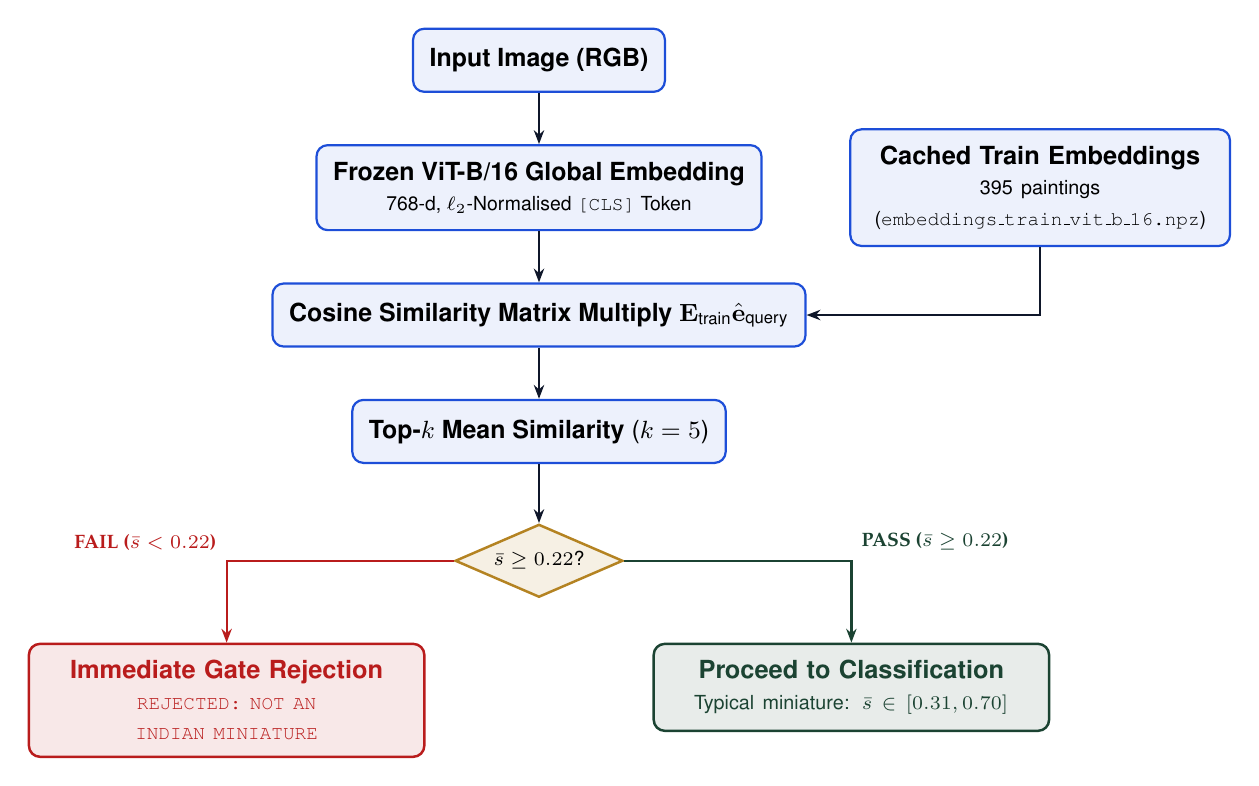
\begin{tikzpicture}[
    node distance=0.65cm and 1.1cm,
    font=\sffamily\small,
    blk/.style={draw=SoftBlue, fill=SoftBlue!8, rounded corners=4pt, align=center, minimum height=0.8cm, inner sep=6pt, line width=0.8pt},
    dec/.style={diamond, aspect=2.3, draw=ImperialGold, fill=ImperialGold!12, align=center, inner sep=2pt, line width=0.9pt},
    rej/.style={draw=AccentRed, fill=AccentRed!10, rounded corners=4pt, align=center, inner sep=6pt, line width=0.9pt, text=AccentRed},
    pas/.style={draw=MughalGreen, fill=MughalGreen!10, rounded corners=4pt, align=center, inner sep=6pt, line width=0.9pt, text=MughalGreen},
    arr/.style={-{Stealth[length=5pt]}, thick, color=ObsidianBlue}
  ]
    \node[blk] (img) {\textbf{Input Image (RGB)}};
    \node[blk, below=of img] (vit) {\textbf{Frozen ViT-B/16 Global Embedding}\\{\scriptsize 768-d, $\ell_2$-Normalised \texttt{[CLS]} Token}};
    \node[blk, right=of vit, text width=4.4cm] (cache) {\textbf{Cached Train Embeddings}\\{\scriptsize 395 paintings (\texttt{embeddings\_train\_vit\_b\_16.npz})}};
    \node[blk, below=of vit] (sim) {\textbf{Cosine Similarity Matrix Multiply} $\mathbf{E}_{\text{train}}\hat{\mathbf{e}}_{\text{query}}$};
    \node[blk, below=of sim] (topk) {\textbf{Top-$k$ Mean Similarity} ($k=5$)};
    \node[dec, below=0.75cm of topk] (gate) {\scriptsize $\bar{s} \ge 0.22$?};
    \node[rej, below left=0.8cm and 0.9cm of gate, text width=4.6cm] (reject) {\textbf{Immediate Gate Rejection}\\{\scriptsize \texttt{REJECTED: NOT AN INDIAN MINIATURE}}};
    \node[pas, below right=0.8cm and 0.9cm of gate, text width=4.6cm] (pass) {\textbf{Proceed to Classification}\\{\scriptsize Typical miniature: $\bar{s} \in [0.31, 0.70]$}};

    \draw[arr] (img) -- (vit);
    \draw[arr] (vit) -- (sim);
    \draw[arr] (cache) |- (sim);
    \draw[arr] (sim) -- (topk);
    \draw[arr] (topk) -- (gate);
    \draw[arr, color=AccentRed] (gate) -| node[above left, font=\scriptsize\bfseries]{FAIL ($\bar{s} < 0.22$)} (reject);
    \draw[arr, color=MughalGreen] (gate) -| node[above right, font=\scriptsize\bfseries]{PASS ($\bar{s} \ge 0.22$)} (pass);
  \end{tikzpicture}%
  }
  \caption{OOD miniature gate: cosine similarity against the training corpus embedding matrix determines whether the input proceeds to classification.}
  \label{fig:ood}
\end{figure}

The gate is implemented in \texttt{BTP/src/ood.py} (\texttt{MiniatureGate}) for the full research pipeline and replicated in \texttt{backend/ml\_bridge/predict.py} for the web inference path.

A frozen ViT-B/16 model (pretrained on ImageNet-21K via the \texttt{timm} library) produces the input image's ${\ell_2}$-normalised 768-dimensional \texttt{[CLS]} token embedding. This vector is compared against precomputed embeddings of all 395 training paintings stored in \texttt{BTP/data/cache/embeddings\_train\_vit\_b\_16.npz} via a single matrix multiply:

\begin{equation}
  \mathbf{s} = \mathbf{E}_{\text{train}}\, \hat{\mathbf{e}}_{\text{query}}, \quad
  \bar{s} = \frac{1}{k} \sum_{j \in \text{top-}k} s_j
  \label{eq:ood}
\end{equation}

where $\mathbf{E}_{\text{train}} \in \mathbb{R}^{395 \times 768}$ is the row-normalised training embedding matrix, $k = 5$, and $\bar{s}$ is the mean top-5 cosine similarity.

\begin{itemize}
  \item \textbf{Web inference gate}: $\bar{s} < 0.22$ triggers rejection with verdict \texttt{REJECTED: NOT AN INDIAN MINIATURE PAINTING}.
  \item \textbf{Full research dual gate}: additionally requires zero-shot CLIP (\texttt{ViT-B/32}) miniature probability $\geq 0.50$ contrasting seven plain-language prompts.
\end{itemize}

Empirical validation confirms: all 169 known val/test miniatures pass (minimum $\bar{s} = 0.305$); all 12 control non-miniatures fail (maximum $\bar{s} = 0.189$).

\begin{importantbox}
  \textbf{Why this gate is essential.} Closed-set softmax heads assign probabilities summing to 100\% across known miniature labels regardless of the input's actual content. Without an OOD gate, a photograph of a dog submitted to the system would receive a confident Mughal attribution, as the dominant training class acts as a catch-all absorber. Temperature Scaling cannot correct out-of-distribution inputs — calibration is defined only on the in-distribution validation set.
\end{importantbox}

\subsection{Stage 2 — High-Resolution Preprocessing and Sliding Windows}

Miniature authenticity is encoded at multiple scales: at the canvas level in overall compositional symmetry and palette, and at the micro-scale in \textit{nim-qalam} stippled shading, \textit{wasli} paper fibre grain, and gold-leaf application patterns. Direct downsampling to $224 \times 224$ destroys micro-scale evidence.

\texttt{BTP/src/preprocessing.py} implements two domain-preserving operations:

\textbf{PaintingPreprocessor}: applies (a) edge-preserving denoising via Non-Local Means (\texttt{fastNlMeansDenoisingColored}) to remove scanner noise while preserving ink outlines; (b) patina-safe white balance via Modified Grey-World scaling blended $0.70 \times \text{original} + 0.30 \times \text{normalised}$ to preserve antique ivory warmth; (c) CLAHE on the CIE-Lab $L^*$ channel with $\gamma = 1.05$ gamma adjustment; and (d) unsharp masking ($I_{\text{sharp}} = I + 1.2 \times (I - \text{GaussBlur}(I))$) to reinforce fine contours.

\textbf{SlidingWindowGenerator}: tiles high-resolution canvases into overlapping $512 \times 512$ windows (stride $256\text{px}$, reflection padding \texttt{BORDER\_REFLECT\_101}) and maps every locally detected bounding box back to global canvas coordinates via affine offset.

\subsection{Stage 3 — Open-Vocabulary Motif Detection}

Iconographic content—courtiers, musicians, deer, peacocks, garden pavilions—provides discriminative evidence for school and period attribution. YOLO-World (\texttt{yolov8s-worldv2.pt}) detects arbitrary text-specified categories without bounding-box training annotations. Thirty plain-English detection prompts (\texttt{DETECTION\_PROMPTS}) cover the principal miniature subject repertoire:

\begin{lstlisting}[language={}, caption={YOLO-World detection prompts for miniature iconography}, label={lst:prompts}]
woman, man, musician, dancer, deer, peacock, turban, crown,
pavilion, canopy, lotus, sword, musical instrument, swing,
lamp, text, horse, bird, tree, flower, water, boat,
elephant, tiger, monkey, dog, rock, sky, cloud, person
\end{lstlisting}

Per-class global non-maximum suppression (IoU $= 0.40$) aggregates detections across overlapping sliding-window tiles. Empirical recall across 564 paintings: turban 96\%, pavilion 95\%, peacock 88\%, 9,609 motif crops extracted in total.

\subsection{Stage 4 — Dual-Branch Feature Fusion}

\begin{figure}[H]
  \centering
  \resizebox{\linewidth}{!}{%
  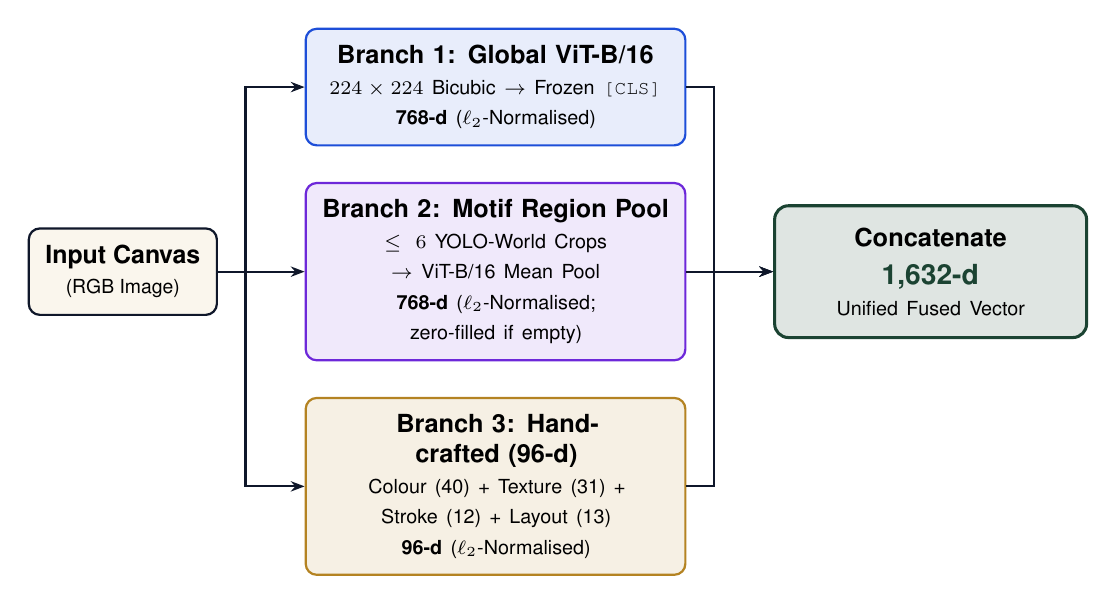
\begin{tikzpicture}[
    node distance=0.6cm and 0.9cm,
    font=\sffamily\small,
    inb/.style={draw=ObsidianBlue, fill=IvoryWhite, rounded corners=4pt, align=center, inner sep=6pt, line width=0.8pt},
    b1/.style={draw=SoftBlue, fill=SoftBlue!10, rounded corners=4pt, align=center, inner sep=6pt, line width=0.8pt, text width=4.4cm},
    b2/.style={draw=PurpleHead, fill=PurpleHead!10, rounded corners=4pt, align=center, inner sep=6pt, line width=0.8pt, text width=4.4cm},
    b3/.style={draw=ImperialGold, fill=ImperialGold!12, rounded corners=4pt, align=center, inner sep=6pt, line width=0.8pt, text width=4.4cm},
    cat/.style={draw=MughalGreen, fill=MughalGreen!14, rounded corners=5pt, align=center, inner sep=8pt, line width=1.1pt, text width=3.4cm},
    arr/.style={-{Stealth[length=5pt]}, thick, color=ObsidianBlue}
  ]
    \node[inb] (canvas) {\textbf{Input Canvas}\\{\scriptsize (RGB Image)}};
    \node[b2, right=1.1cm of canvas] (br2) {\textbf{Branch 2: Motif Region Pool}\\{\scriptsize $\le 6$ YOLO-World Crops $\rightarrow$ ViT-B/16 Mean Pool}\\{\scriptsize \textbf{768-d} ($\ell_2$-Normalised; zero-filled if empty)}};
    \node[b1, above=0.45cm of br2] (br1) {\textbf{Branch 1: Global ViT-B/16}\\{\scriptsize $224\times224$ Bicubic $\rightarrow$ Frozen \texttt{[CLS]}}\\{\scriptsize \textbf{768-d} ($\ell_2$-Normalised)}};
    \node[b3, below=0.45cm of br2] (br3) {\textbf{Branch 3: Handcrafted (96-d)}\\{\scriptsize Colour (40) + Texture (31) + Stroke (12) + Layout (13)}\\{\scriptsize \textbf{96-d} ($\ell_2$-Normalised)}};
    \node[cat, right=1.1cm of br2] (concat) {\textbf{Concatenate}\\[0.1cm]{\normalsize\bfseries\color{MughalGreen} 1,632-d}\\{\scriptsize Unified Fused Vector}};

    \draw[arr] (canvas.east) -- ++(0.35,0) |- (br1.west);
    \draw[arr] (canvas.east) -- (br2.west);
    \draw[arr] (canvas.east) -- ++(0.35,0) |- (br3.west);
    \draw[arr] (br1.east) -- ++(0.35,0) |- (concat.west);
    \draw[arr] (br2.east) -- (concat.west);
    \draw[arr] (br3.east) -- ++(0.35,0) |- (concat.west);
  \end{tikzpicture}%
  }
  \caption{Dual-branch 1,632-dimensional feature fusion pipeline: global ViT-B/16 embedding (768-d), region-pooled motif-crop embedding (768-d), and 96 handcrafted art-historical descriptors. Each branch is independently ${\ell_2}$-normalised before concatenation.}
  \label{fig:fusion}
\end{figure}

The 1,632-dimensional fused representation $\mathbf{f} = [\hat{\mathbf{e}}_{\text{global}}; \hat{\mathbf{e}}_{\text{region}}; \hat{\mathbf{d}}_{\text{craft}}]$ is constructed from three branches, each independently ${\ell_2}$-normalised to prevent magnitude dominance:

\subsubsection{Branch 1 — Global ViT-B/16 Embedding (768-d)}
The input canvas is resized to $224 \times 224$ bicubic, normalised with ImageNet mean/std, and forwarded through the frozen ViT-B/16 backbone. The \texttt{[CLS]} token output is ${\ell_2}$-normalised.

\subsubsection{Branch 2 — Region-Pooled Motif Crop Embedding (768-d)}
Up to 6 YOLO-World motif crops are individually embedded by the same frozen ViT-B/16 backbone. The resulting embeddings are mean-pooled. If no motifs are detected, this branch is set to the zero vector, contributing no information while preserving the fixed 1,632-d input dimension for the downstream classifier.

\subsubsection{Branch 3 — Handcrafted Art-Historical Descriptors (96-d)}

\begin{table}[H]
  \centering
  \caption{Handcrafted feature sub-branches with dimensions and art-historical motivations.}
  \label{tab:features}
  \rowcolors{2}{IvoryWhite}{white}
  \begin{tabularx}{\linewidth}{L{2.8cm} C{0.8cm} X}
    \toprule
    \rowcolor{MughalGreen!15}
    \textbf{Sub-Branch} & \textbf{Dim} & \textbf{Signal}\\
    \midrule
    Colour \& Mineral Pigments &
      40 &
      $16$-bin HSV hue + $8$-bin saturation + $8$-bin value histograms (32-d); CIE-Lab channel means and standard deviations (6-d); Gold Leaf Index ($H \in [15,35]$, $S \geq 100$, $V \geq 150$) distinguishing gilded Mughal and Deccani manuscripts (1-d); Mineral Lac/Hinglu Red Index ($H \leq 10$ or $\geq 170$, $S \geq 120$, $V \geq 100$) for Mewar flat-ground pigments (1-d).\\
    \midrule
    Micro-texture \& Paper Grain &
      31 &
      GLCM statistics (contrast, dissimilarity, homogeneity, energy, correlation) at distances $[1,3]$ over four angles (5-d); Uniform LBP ($P=8$, $R=1$) capturing \textit{wasli} fibre and stippled shading (10-d); Gabor filter bank mean and std across two spatial frequencies and four orientations (16-d).\\
    \midrule
    Stroke \& Line Morphology &
      12 &
      Canny edge density, normalised mean and maximum contour arc length, contour density (4-d); 8-bin Sobel gradient orientation histogram masked to edge pixels (8-d).\\
    \midrule
    Spatial Composition &
      13 &
      3$\times$3 Rule-of-Thirds normalised luminance grid (9-d); horizontal and vertical mirror symmetry scores (2-d); centre-of-mass focal offset $(x, y) \in [-0.5, +0.5]^2$ (2-d).\\
    \midrule
    \textbf{Total} & \textbf{96} & \\
    \bottomrule
  \end{tabularx}
\end{table}

\subsection{Stage 5 — Multi-Head Neural Classifier}

\begin{figure}[H]
  \centering
  \resizebox{\linewidth}{!}{%
  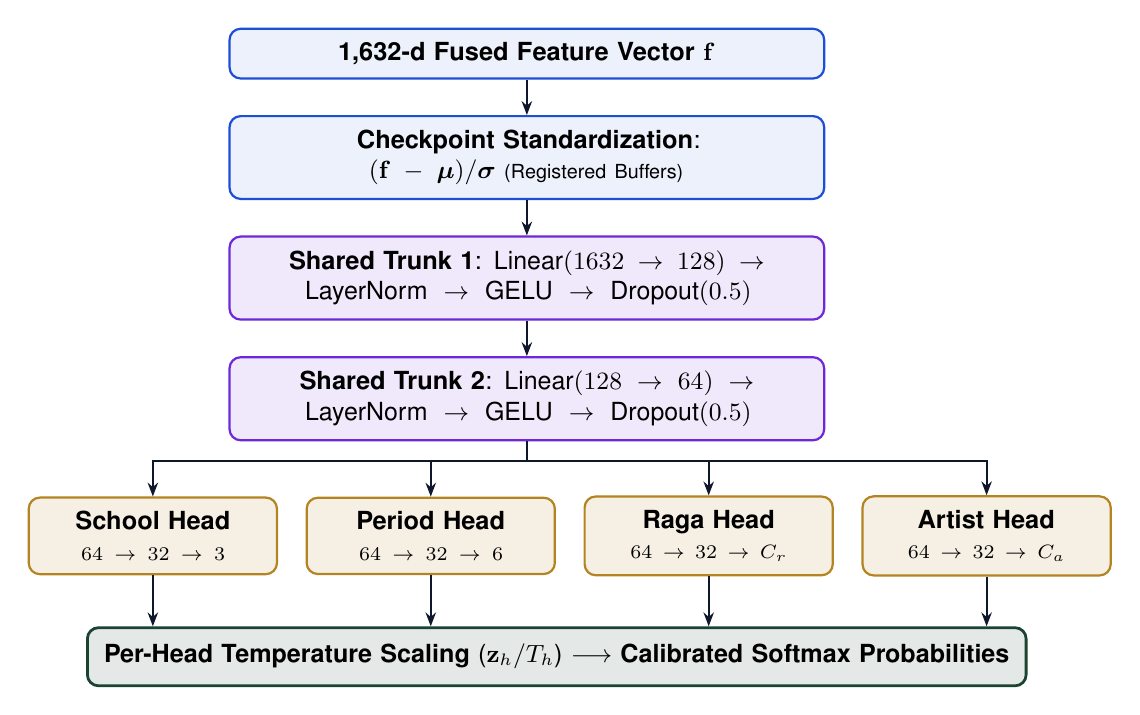
\begin{tikzpicture}[
    node distance=0.5cm and 0.65cm,
    font=\sffamily\small,
    blk/.style={draw=SoftBlue, fill=SoftBlue!8, rounded corners=4pt, align=center, inner sep=5pt, line width=0.8pt},
    trk/.style={draw=PurpleHead, fill=PurpleHead!10, rounded corners=4pt, align=center, inner sep=5pt, line width=0.8pt, text width=7.2cm},
    hd/.style={draw=ImperialGold, fill=ImperialGold!12, rounded corners=4pt, align=center, inner sep=5pt, line width=0.8pt, text width=2.8cm},
    cal/.style={draw=MughalGreen, fill=MughalGreen!12, rounded corners=4pt, align=center, inner sep=6pt, line width=1pt, text width=11.5cm},
    arr/.style={-{Stealth[length=5pt]}, thick, color=ObsidianBlue}
  ]
    \node[blk, text width=7.2cm] (in) {\textbf{1,632-d Fused Feature Vector} $\mathbf{f}$};
    \node[blk, below=0.45cm of in, text width=7.2cm] (std) {\textbf{Checkpoint Standardization}: $(\mathbf{f} - \boldsymbol{\mu}) / \boldsymbol{\sigma}$ {\scriptsize (Registered Buffers)}};
    \node[trk, below=0.45cm of std] (t1) {\textbf{Shared Trunk 1}: $\text{Linear}(1632 \to 128) \to \text{LayerNorm} \to \text{GELU} \to \text{Dropout}(0.5)$};
    \node[trk, below=0.45cm of t1] (t2) {\textbf{Shared Trunk 2}: $\text{Linear}(128 \to 64) \to \text{LayerNorm} \to \text{GELU} \to \text{Dropout}(0.5)$};

    \node[hd, below=0.7cm of t2, xshift=-4.75cm] (h1) {\textbf{School Head}\\{\scriptsize $64 \to 32 \to 3$}};
    \node[hd, right=0.35cm of h1] (h2) {\textbf{Period Head}\\{\scriptsize $64 \to 32 \to 6$}};
    \node[hd, right=0.35cm of h2] (h3) {\textbf{Raga Head}\\{\scriptsize $64 \to 32 \to C_r$}};
    \node[hd, right=0.35cm of h3] (h4) {\textbf{Artist Head}\\{\scriptsize $64 \to 32 \to C_a$}};

    \node[cal, below=0.65cm of h2, xshift=1.6cm] (ts) {\textbf{Per-Head Temperature Scaling} ($\mathbf{z}_h / T_h$) $\longrightarrow$ \textbf{Calibrated Softmax Probabilities}};

    \draw[arr] (in) -- (std);
    \draw[arr] (std) -- (t1);
    \draw[arr] (t1) -- (t2);
    \draw[arr] (t2.south) -- ++(0,-0.25) -| (h1.north);
    \draw[arr] (t2.south) -- ++(0,-0.25) -| (h2.north);
    \draw[arr] (t2.south) -- ++(0,-0.25) -| (h3.north);
    \draw[arr] (t2.south) -- ++(0,-0.25) -| (h4.north);
    \draw[arr] (h1.south) -- (h1.south |- ts.north);
    \draw[arr] (h2.south) -- (h2.south |- ts.north);
    \draw[arr] (h3.south) -- (h3.south |- ts.north);
    \draw[arr] (h4.south) -- (h4.south |- ts.north);
  \end{tikzpicture}%
  }
  \caption{Multi-head classifier architecture: a shared two-layer trunk processes the 1,632-d input, then four task-specific heads produce logits for School, Period, Raga, and Artist classification.}
  \label{fig:multihead}
\end{figure}

Implemented in \texttt{BTP/src/multihead\_classifier.py}, the \texttt{MultiHeadMiniatureClassifier} maps the 1,632-d fused vector through a standardised shared trunk, then branches into four heads:

\begin{equation}
  \mathbf{z}_h = W_{h2}\,\sigma\!\left(W_{h1}\,\sigma\!\left(W_{t2}\,\sigma\!\left(W_{t1}\,\frac{\mathbf{f} - \boldsymbol{\mu}}{\boldsymbol{\sigma}}\right)\right)\right), \quad h \in \{\text{school, period, raga, artist}\}
\end{equation}

where $\sigma$ denotes GELU activation, Dropout is applied after each activation ($p = 0.5$ in trunk, $p = 0.25$ in heads), and LayerNorm follows each trunk linear layer. Training-split per-feature mean $\boldsymbol{\mu}$ and standard deviation $\boldsymbol{\sigma}$ are stored as PyTorch buffers inside the \texttt{.pt} checkpoint so they are automatically applied at inference without caller involvement.

Training hyperparameters: AdamW ($\text{lr} = 10^{-3}$, $\lambda = 10^{-2}$), CosineAnnealingLR, $H = 128$, batch size 16, early stopping patience 12. Balanced class-weighted cross-entropy loss:

\begin{equation}
  \mathcal{L} = \sum_{h} \mathcal{L}_{\text{CE}}(\mathbf{z}_h, y_h;\, \mathbf{w}_h^{\text{balanced}}, \texttt{ignore\_index}=-100)
\end{equation}

\subsection{Stage 6 — Post-Hoc Temperature Scaling Calibration}

Raw logits from trained neural classifiers systematically overstate certainty. For each head $h$, a scalar temperature $T_h > 0$ is fitted on the 85-painting validation set by minimising Negative Log-Likelihood via bounded scalar optimisation ($\log T_h \in [\ln 0.05, \ln 20.0]$):

\begin{equation}
  P_{\text{cal}}(y = c \mid \mathbf{x}) = \frac{\exp(z_c / T_h)}{\sum_j \exp(z_j / T_h)}
  \label{eq:tempcal}
\end{equation}

Because division by a positive scalar is strictly monotonic, Temperature Scaling never alters the top-1 prediction — it solely adjusts probability magnitudes.

\begin{table}[H]
  \centering
  \caption{Per-head calibration results on the 85-painting validation set.}
  \label{tab:calibration}
  \rowcolors{2}{IvoryWhite}{white}
  \begin{tabularx}{\linewidth}{L{2.4cm} C{1.5cm} C{1.6cm} C{1.6cm} C{1.6cm} C{1.6cm}}
    \toprule
    \rowcolor{MughalGreen!15}
    \textbf{Head} & \textbf{Temp $T$} & \textbf{ECE Pre} & \textbf{ECE Post} & \textbf{Brier Pre} & \textbf{Brier Post}\\
    \midrule
    School  & 1.518 & 6.93\% & 4.87\% & 0.1388 & 0.1248\\
    Period  & 0.861 & 10.88\%& 9.75\% & 0.4338 & 0.4223\\
    Raga    & 0.828 & 6.27\% & 8.44\% & 0.1299 & 0.1321\\
    Artist  & 0.054 & 1.16\% & 3.57\% & 0.0437 & 0.0476\\
    \bottomrule
  \end{tabularx}
\end{table}

Pooled reliability verification: predictions with calibrated confidence $\geq 0.70$ ($n = 180$) achieve 94.4\% observed precision; the $[0.60, 0.80)$ confidence band ($n = 19$, mean confidence 73.6\%) achieves 68.4\% observed precision.

\subsection{Stage 7 — Visual Telemetry, VLM Cross-Check, and Active Learning}

\subsubsection{Real-Time Telemetry and Grounded Synthesis}

\texttt{backend/ml\_bridge/predict.py} computes six real-time scalar metrics from the raw image (without loading the ML checkpoint): \texttt{gold\_pigment\_index}, \texttt{mineral\_red\_index}, \texttt{horizontal\_symmetry}, \texttt{vertical\_symmetry}, \texttt{focal\_offset\_x/y}, and \texttt{texture\_entropy} (log\textsubscript{10} Laplacian variance). These metrics are returned alongside the classifier output and displayed in the Visual Features panel of the frontend.

\subsubsection{Qwen 2.5-VL Multimodal Judge}

In the full research pipeline, Qwen~2.5-VL~7B (served via local Ollama) inspects the painting alongside detected motif crops and a Retrieval-Augmented knowledge dossier assembled from Sanskrit \textit{Dhyana} verse databases, school characteristic profiles, and period pigment records. The VLM enforces grammar-constrained JSON schema decoding with mandatory \texttt{"uncertain"} abstention when evidence is insufficient, and triggers cross-check routing whenever its top prediction disagrees with the classifier or its own calibrated confidence falls below 0.70.

\subsubsection{Human-in-the-Loop Active Retraining}

Expert curator corrections submitted through the web interface's Expert Review Modal are stored in \texttt{backend/data/feedback.json} and the MongoDB \texttt{Feedback} collection. The CLI tool \texttt{review\_feedback.py retrain} reads these corrections, overrides split labels, and triggers retraining, closing the loop between domain expertise and model improvement.

%==============================================================
\section{Backend Architecture and ML Bridge}
\label{sec:backend}
%==============================================================

The backend is a Node.js (ES Module) Express.js application that orchestrates image uploads, bridges requests to the Python ML runtime, and persists predictions.

\subsection{Server Configuration and Middleware}

\texttt{backend/server.js} initialises in the following order:

\begin{enumerate}
  \item Load environment variables from \texttt{.env} via \texttt{dotenv}.
  \item Configure CORS with \texttt{origin: true}, \texttt{credentials: true}, accommodating both the local Vite dev server (port 5173) and the deployed Vercel frontend origin.
  \item Mount \texttt{express.json()} and \texttt{express.urlencoded()} body parsers.
  \item Statically serve \texttt{backend/uploads/} at \texttt{/uploads} and \texttt{BTP/data/raw/images/} at \texttt{/samples}.
  \item Attempt MongoDB connection (\texttt{serverSelectionTimeoutMS: 2000}); on failure, log a notice and continue in JSON-only mode.
  \item Register all API route modules and start listening on \texttt{PORT} or 5000.
\end{enumerate}

\subsection{The Node-to-Python Machine Learning Bridge}

The central architectural challenge is bridging a JavaScript runtime to a PyTorch checkpoint. The solution is a \emph{child-process subprocess interface}.

\begin{figure}[H]
  \centering
  \resizebox{\linewidth}{!}{%
  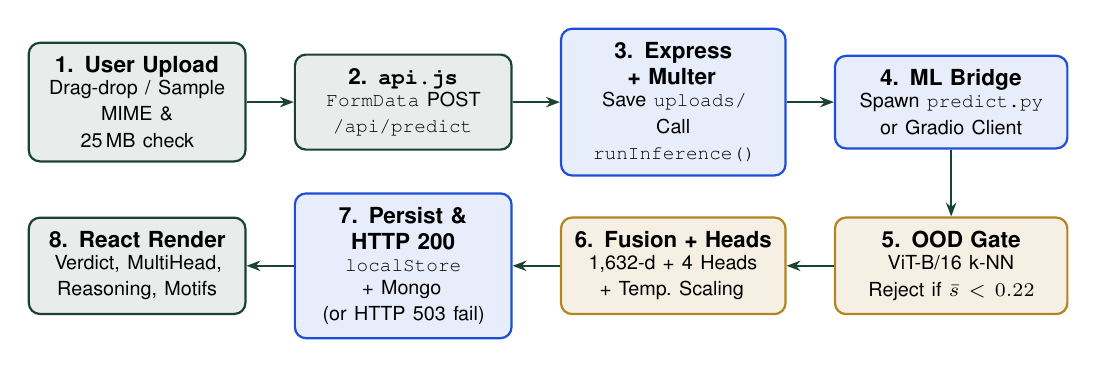
\begin{tikzpicture}[
    node distance=0.55cm and 0.6cm,
    font=\sffamily\footnotesize,
    stepbox/.style={draw=ObsidianBlue, fill=white, rounded corners=4pt, align=center, inner sep=5pt, minimum height=0.85cm, line width=0.8pt},
    arr/.style={-{Stealth[length=5pt]}, thick, color=MughalGreen}
  ]
    \node[stepbox, fill=MughalGreen!10, draw=MughalGreen, text width=2.4cm] (s1) {\textbf{1. User Upload}\\{\scriptsize Drag-drop / Sample\\MIME \& 25\,MB check}};
    \node[stepbox, fill=MughalGreen!10, draw=MughalGreen, right=of s1, text width=2.4cm] (s2) {\textbf{2. \texttt{api.js}}\\{\scriptsize \texttt{FormData} POST\\\texttt{/api/predict}}};
    \node[stepbox, fill=SoftBlue!10, draw=SoftBlue, right=of s2, text width=2.5cm] (s3) {\textbf{3. Express + Multer}\\{\scriptsize Save \texttt{uploads/}\\Call \texttt{runInference()}}};
    \node[stepbox, fill=SoftBlue!10, draw=SoftBlue, right=of s3, text width=2.6cm] (s4) {\textbf{4. ML Bridge}\\{\scriptsize Spawn \texttt{predict.py}\\or Gradio Client}};
    \node[stepbox, fill=ImperialGold!12, draw=ImperialGold, below=0.85cm of s4, text width=2.6cm] (s5) {\textbf{5. OOD Gate}\\{\scriptsize ViT-B/16 k-NN\\Reject if $\bar{s} < 0.22$}};
    \node[stepbox, fill=ImperialGold!12, draw=ImperialGold, left=of s5, text width=2.5cm] (s6) {\textbf{6. Fusion + Heads}\\{\scriptsize 1,632-d + 4 Heads\\+ Temp.\ Scaling}};
    \node[stepbox, fill=SoftBlue!10, draw=SoftBlue, left=of s6, text width=2.4cm] (s7) {\textbf{7. Persist \& HTTP 200}\\{\scriptsize \texttt{localStore} + Mongo\\(or HTTP 503 fail)}};
    \node[stepbox, fill=MughalGreen!10, draw=MughalGreen, left=of s7, text width=2.4cm] (s8) {\textbf{8. React Render}\\{\scriptsize Verdict, MultiHead,\\Reasoning, Motifs}};

    \draw[arr] (s1) -- (s2);
    \draw[arr] (s2) -- (s3);
    \draw[arr] (s3) -- (s4);
    \draw[arr] (s4) -- (s5);
    \draw[arr] (s5) -- (s6);
    \draw[arr] (s6) -- (s7);
    \draw[arr] (s7) -- (s8);
  \end{tikzpicture}%
  }
  \caption{End-to-end command and data flow: from user image upload through the Express API, the Node-to-Python subprocess bridge, the seven-stage ML pipeline, to the structured JSON response rendered across frontend components.}
  \label{fig:dataflow}
\end{figure}

\textbf{Local runner} (\texttt{backend/ml\_bridge/runner.js}): \texttt{getPythonCommand()} probes for the project's virtual environment at \texttt{../../.venv/Scripts/python.exe} (falling back to system Python). \texttt{runInference(imagePath)} spawns:

\begin{lstlisting}[language={}, caption={ML bridge subprocess command}, label={lst:bridge}]
<pythonExe> backend/ml_bridge/predict.py --image <imagePath>
\end{lstlisting}

with \texttt{cwd} set to the repository root and \texttt{PYTHONIOENCODING=utf-8}. It accumulates stdout chunks, locates the outermost JSON object using brace-matching, and resolves the promise with the parsed prediction object.

\begin{warningbox}
  \textbf{Fail-Loud Guarantee.} If \texttt{predict.py} cannot import \texttt{torch}, locate \texttt{multihead\_fused\_classifier.pt}, or complete any stage, it prints \texttt{\{"error": "...", "model\_running": false\}} to stdout and exits with code 1. \texttt{routes/predict.js} intercepts \texttt{mlResult.model\_running === false} and returns HTTP 503 Service Unavailable. The frontend displays an explicit, user-readable error notice. No simulated, cached, or fallback predictions are ever served.
\end{warningbox}

\textbf{Cloud runner} (\texttt{backend/ml\_bridge/runner1.js}): connects to the Hugging Face Space \texttt{ArkaKGP/mughal-art-classifier} via \texttt{@gradio/client}, reads the uploaded file into a \texttt{Blob}, and invokes the remote \texttt{/predict} endpoint. The returned payload is structurally identical to the local runner's output.

\subsection{REST API Endpoints}

\begin{longtable}{L{3.0cm} C{1.2cm} L{3.0cm} L{5.5cm}}
  \caption{REST API endpoints exposed by the Express server.}
  \label{tab:api}\\
  \toprule
  \rowcolor{MughalGreen!15}
  \textbf{Endpoint} & \textbf{Method} & \textbf{Handler} & \textbf{Behaviour}\\
  \midrule
  \endfirsthead
  \multicolumn{4}{c}{\textit{Table \ref{tab:api} continued}}\\
  \toprule
  \rowcolor{MughalGreen!15}
  \textbf{Endpoint} & \textbf{Method} & \textbf{Handler} & \textbf{Behaviour}\\
  \midrule
  \endhead
  \bottomrule
  \endfoot
  \texttt{/api/health}         & GET  & \texttt{server.js}        & Service heartbeat; returns \texttt{mongoConnected} flag.\\
  \texttt{/api/predict}        & POST & \texttt{routes/predict.js} & Accepts \texttt{multipart/form-data} (\texttt{image} field, $\leq$25\,MB, JPEG/PNG/WebP). Multer saves to \texttt{uploads/}. Calls \texttt{runInference}, persists to \texttt{localStore} + MongoDB, returns full JSON + \texttt{analysisId}.\\
  \texttt{/api/predict-sample} & POST & \texttt{routes/predict.js} & Accepts \texttt{\{sampleFilename\}}. Resolves path in curated dataset, calls \texttt{runInference}, returns result with \texttt{/samples/<filename>} URL.\\
  \texttt{/api/samples}        & GET  & \texttt{routes/samples.js} & Returns 6 curated benchmark paintings with disk-presence check and \texttt{/samples/...} URLs.\\
  \texttt{/api/history}        & GET  & \texttt{routes/history.js} & Returns latest $\leq$20 analysis records in reverse-chronological order.\\
  \texttt{/api/feedback}       & GET/POST & \texttt{routes/feedback.js} & Lists or records expert ground-truth corrections. Writes to \texttt{data/feedback.json} and MongoDB \texttt{Feedback} collection.\\
  \texttt{/api/stats}          & GET  & \texttt{routes/stats.js}   & Reads \texttt{BTP/reports/final\_evaluation.json}; serves head accuracies, Macro F1s, dataset counts, and pipeline specs. Safe fallback defaults if report absent.\\
\end{longtable}

\subsection{Data Models and Fallback Storage}

\textbf{Mongoose schemas}: \texttt{backend/models/Analysis.js} captures the full analysis record — image path, four-head prediction objects, visual feature telemetry, detected motifs, VLM cross-check block, and timestamp. \texttt{backend/models/Feedback.js} captures expert corrections with a foreign-key reference to the \texttt{Analysis} collection.

\textbf{JSON fallback store} (\texttt{backend/data/localStore.js}): synchronous JSON persistence ensuring zero-configuration operation without MongoDB. Creates \texttt{data/history.json} and \texttt{data/feedback.json} on first run; provides \texttt{addAnalysis()}, \texttt{getHistory()}, \texttt{addFeedback()}, and \texttt{getFeedback()} helpers.

%==============================================================
\section{Frontend Architecture and User Interface}
\label{sec:frontend}
%==============================================================

The frontend is a React~19 / Vite~8 / Tailwind CSS~v4 single-page application styled around a museum-grade aesthetic with globally switchable Day and Night themes.

\subsection{Design Principles}

Two principles governed every interface decision:

\begin{enumerate}
  \item \textbf{Subject-appropriate visual language.} Indian miniature scholarship demands an environment that communicates authority and historical depth. The Day Theme (Ivory Parchment backgrounds, Mughal Green accents, antique gold highlights) evokes a manuscript reading room; the Night Theme (Obsidian surface, Imperial Gold accents) a museum gallery after hours.
  \item \textbf{Multi-dimensional ML output legibility.} The system produces four simultaneous calibrated probability distributions, six scalar telemetry metrics, up to six detected motifs, a consensus or discrepancy verdict, and a prose reasoning paragraph. Each output class requires a dedicated display surface.
\end{enumerate}

Typography: \textbf{Cinzel} (a Roman serif recalling Devanagari proportions) for display headings and category labels; \textbf{Plus Jakarta Sans} for all body text and UI controls.

\subsection{Build, Proxy, and Deployment Configuration}

\begin{table}[H]
  \centering
  \caption{Configuration files and their roles in the frontend build pipeline.}
  \label{tab:config}
  \rowcolors{2}{IvoryWhite}{white}
  \begin{tabularx}{\linewidth}{L{3.5cm} X}
    \toprule
    \rowcolor{MughalGreen!15}
    \textbf{File} & \textbf{Role}\\
    \midrule
    \texttt{frontend/package.json}     & Runtime: \texttt{react}~19.3, \texttt{react-dom}~19.3, \texttt{lucide-react}, \texttt{canvas-confetti}. Dev: \texttt{vite}~8.3, \texttt{@vitejs/plugin-react}, \texttt{@tailwindcss/vite}~4.3, \texttt{oxlint}.\\
    \texttt{frontend/index.html}       & HTML shell loading Cinzel and Plus Jakarta Sans from Google Fonts; mounts React into \texttt{\#root}.\\
    \texttt{frontend/vite.config.js}   & Proxies \texttt{/api}, \texttt{/uploads}, \texttt{/samples} to \texttt{http://localhost:5000} in development; enables relative-path API calls that work identically in production.\\
    \texttt{frontend/vercel.json}      & Sets framework to \texttt{vite}; adds catch-all SPA rewrite (\texttt{/(.*) -> /index.html}) to prevent CDN 404s on deep-link navigation.\\
    \bottomrule
  \end{tabularx}
\end{table}

\subsection{State Management and Service Layer}

\textbf{\texttt{frontend/src/context/ThemeContext.jsx}}: Provides \texttt{ThemeProvider} and \texttt{useTheme()} (\texttt{theme}, \texttt{isNight}, \texttt{toggleTheme}). Persists preference in \texttt{localStorage} under \texttt{'mughal\_theme'} and toggles \texttt{day-theme}/\texttt{night-theme} on \texttt{document.documentElement}. All Tailwind utilities and CSS custom properties resolve against the active class.

\textbf{\texttt{frontend/src/services/api.js}}: Centralises all HTTP communication. Reads \texttt{VITE\_API\_URL} from the build environment (Vercel deployment) or defaults to empty string (Vite proxy). Exports six typed async functions:

\begin{table}[H]
  \centering
  \caption{API service layer functions and their HTTP contracts.}
  \label{tab:apiservice}
  \rowcolors{2}{IvoryWhite}{white}
  \begin{tabularx}{\linewidth}{L{4.2cm} C{1.0cm} L{2.4cm} X}
    \toprule
    \rowcolor{MughalGreen!15}
    \textbf{Function} & \textbf{Verb} & \textbf{Endpoint} & \textbf{Purpose}\\
    \midrule
    \texttt{uploadAndAnalyzeImage(file)} & POST & \texttt{/api/predict} & Wraps file in \texttt{FormData}, sends as \texttt{multipart/form-data}.\\
    \texttt{analyzeSamplePainting(fn)}   & POST & \texttt{/api/predict-sample} & Sends \texttt{\{sampleFilename\}} JSON.\\
    \texttt{fetchSamplePaintings()}      & GET  & \texttt{/api/samples}        & Retrieves curated benchmark gallery.\\
    \texttt{submitExpertFeedback(p)}     & POST & \texttt{/api/feedback}       & Submits curator correction payload.\\
    \texttt{fetchAnalysisHistory(n)}     & GET  & \texttt{/api/history}        & Retrieves last $n$ analysis records.\\
    \texttt{fetchPipelineStats()}        & GET  & \texttt{/api/stats}          & Retrieves benchmark metrics for Hero Section.\\
    \bottomrule
  \end{tabularx}
\end{table}

\textbf{\texttt{frontend/src/App.jsx}}: Root state orchestrator. Manages \texttt{samples}, \texttt{stats}, \texttt{selectedImage}, \texttt{isAnalyzing}, \texttt{analysisResult}, \texttt{errorMessage}, and three modal/drawer flags. On mount, fetches samples and stats concurrently. On analysis trigger, sets \texttt{isAnalyzing = true}, calls the appropriate API function, stores the result, and smooth-scrolls to the results section via \texttt{resultsRef}.

\subsection{Component Breakdown}

\subsubsection{Navbar}
Sticky \texttt{backdrop-blur-md} navigation bar rendering the project logo, an \texttt{Architecture} modal trigger, a \texttt{History} drawer trigger, and a Day/Night theme toggle with animated sun/moon icon transition.

\begin{figure}[H]
  \centering
  \screenshotorplaceholder{fig_ui_home}
  \caption{Home page showing the navigation bar, hero statistics strip, drag-and-drop image uploader, and curated sample gallery. The Day Theme (Ivory Parchment and Mughal Green) is active.}
  \label{fig:uihome}
\end{figure}

\subsubsection{HeroSection}
Renders the project title, tagline, and a four-card live benchmark statistics strip sourced from \texttt{/api/stats}: School Accuracy (90.5\%), Raga Identification (90.5\%), Period Attribution (66.1\%), and VLM Judge status (Calibrated). Shimmer skeleton placeholders appear while stats are loading.

\subsubsection{ImageUploader}
Implements both drag-and-drop (via \texttt{dragover}, \texttt{dragleave}, \texttt{drop} event listeners) and click-to-browse (hidden \texttt{<input type="file">}) file selection. Validates MIME type (JPEG, PNG, WebP) and file size ($\leq 25$\,MB) before updating state. Generates an instant client-side preview via \texttt{URL.createObjectURL()}. Disables submission and shows a \texttt{Loader2} spinner while \texttt{isAnalyzing} is true.

\subsubsection{SampleGallery}
Displays six curated benchmark paintings in a responsive three-column grid. Each card shows the painting thumbnail, a School pill, an optional Gold Leaf badge, the historical period label, an art-historical summary sentence, and a one-click \textbf{Analyze This Painting} button triggering \texttt{analyzeSamplePainting(sample.filename)}.

\subsubsection{VerdictBanner}
The primary authentication result display, implemented in three distinct visual states:

\begin{itemize}
  \item \textbf{Gate Rejected} (\texttt{is\_miniature === false}): Crimson banner with \texttt{GATE REJECT} stamp, the OOD gate's cosine similarity score, and an explanatory note.
  \item \textbf{Mughal Confirmed} (\texttt{is\_mughal === true}): Green-gold banner with \texttt{VERDICT: YES} stamp and an animated confidence progress bar. When confidence $\geq 80\%$, \texttt{canvas-confetti} triggers a celebration burst.
  \item \textbf{Alternative School} (\texttt{is\_mughal === false}): Amber banner with \texttt{VERDICT: NO} stamp naming the attributed school.
\end{itemize}

\begin{figure}[H]
  \centering
  \screenshotorplaceholder{fig_ui_verdict}
  \caption{VerdictBanner in Mughal-confirmed state: green-gold banner, VERDICT: YES stamp, calibrated confidence bar. The confetti celebration fires when confidence exceeds 80\%.}
  \label{fig:uiverdict}
\end{figure}

\subsubsection{MultiHeadCards}
A 2$\times$2 grid rendering one card per classification head (Artistic School, Historical Period, Raga/Musical Mode, Artist Attribution). Each card displays the top-1 prediction prominently, a temperature-calibrated confidence badge, and a sorted top-3 probability distribution as colour-coded bar charts.

\begin{figure}[H]
  \centering
  \screenshotorplaceholder{fig_ui_multihead}
  \caption{MultiHeadCards: four classification heads rendered as probability distribution cards. Temperature-calibrated confidence values are shown beneath each top prediction.}
  \label{fig:uimultihead}
\end{figure}

\subsubsection{ArtHistorianReasoning}
Renders the Multimodal LLM Reasoning panel from \texttt{result.llm\_reasoning}: a consensus badge, an Art-Historical Synthesis prose block, and two side-by-side bulleted panels (Stylistic \& Brushwork Observations; Historical Atelier \& Epoch Markers).

\begin{figure}[H]
  \centering
  \screenshotorplaceholder{fig_ui_reasoning}
  \caption{Art-Historian Reasoning panel showing the consensus badge, synthesised prose reasoning, stylistic observations, and epoch markers panels.}
  \label{fig:uireasoning}
\end{figure}

\subsubsection{VisualFeaturesCard}
Displays four scalar telemetry tiles (Gold Leaf Index, Mineral Red Index, Canvas Symmetry, Texture Detail) with threshold-based interpretation labels, and a conditional YOLO-World detected motifs pill grid.

\begin{figure}[H]
  \centering
  \screenshotorplaceholder{fig_ui_features}
  \caption{VisualFeaturesCard: pigment telemetry tiles and YOLO-World detected motif pills with per-object confidence percentages.}
  \label{fig:uifeatures}
\end{figure}

\subsubsection{ArchitectureModal}
Full-screen backdrop modal describing all seven system phases from sliding-window preprocessing through human-in-the-loop active retraining.

\subsubsection{HistoryDrawer}
Slide-over right drawer querying \texttt{GET /api/history} on open. Lists past analyses with thumbnails, verdict pills, confidence, filename, and period. Clicking any entry restores both the image preview and the full results dashboard without re-running inference.

\begin{figure}[H]
  \centering
  \screenshotorplaceholder{fig_ui_history}
  \caption{HistoryDrawer open: past analyses listed with verdict pills, confidence values, and thumbnail previews. Clicking any entry restores the full dashboard.}
  \label{fig:uihistory}
\end{figure}

\subsubsection{ExpertReviewModal}
Human-in-the-loop correction dialog. The curator selects the target head, reads the model's current prediction (read-only), enters the ground-truth label, reviewer name, and art-historical notes, and submits via \texttt{POST /api/feedback}.

%==============================================================
\section{End-to-End Integration and Data Flow}
\label{sec:integration}
%==============================================================

\subsection{Request Lifecycle}

The complete lifecycle of a user uploading a painting and receiving results is as follows:

\begin{enumerate}
  \item The user drops a JPEG/PNG/WebP file onto \texttt{ImageUploader}. The component validates MIME type and size, generates a client-side preview, and displays file metadata.
  \item The user clicks \textbf{Analyze Painting}. \texttt{App.jsx} sets \texttt{isAnalyzing = true} and calls \texttt{uploadAndAnalyzeImage(file)}.
  \item \texttt{api.js} constructs \texttt{FormData} with the file attached under \texttt{image} and POSTs to \texttt{/api/predict}.
  \item \texttt{routes/predict.js} receives the request. Multer saves the file to \texttt{backend/uploads/}. The route calls \texttt{runInference(imagePath)}.
  \item \texttt{ml\_bridge/runner.js} spawns \texttt{python backend/ml\_bridge/predict.py --image <path>} with \texttt{PYTHONIOENCODING=utf-8}.
  \item The Python process runs all seven pipeline stages (OOD gate, preprocessing, motif detection, feature fusion, classification, temperature scaling, telemetry synthesis) and prints the structured JSON result to stdout.
  \item \texttt{runner.js} captures stdout, extracts and parses the JSON block, and resolves the Promise with the prediction object.
  \item The route saves the record to \texttt{localStore.js} and MongoDB (if connected) and responds with HTTP~200 and the full result object including \texttt{analysisId}.
  \item \texttt{api.js} returns the parsed response to \texttt{App.jsx}, which stores it in \texttt{analysisResult}, clears \texttt{isAnalyzing}, and smooth-scrolls to the results section.
  \item React re-renders all result components, and if the painting is Mughal with confidence $\geq 80\%$, \texttt{canvas-confetti} fires.
\end{enumerate}

\subsection{Sample Analysis Path}

For gallery paintings, the user clicks \textbf{Analyze This Painting} in \texttt{SampleGallery}. \texttt{App.jsx} calls \texttt{analyzeSamplePainting(sample.filename)}, which POSTs \texttt{\{sampleFilename\}} to \texttt{/api/predict-sample}. The route resolves the filename to an absolute path in \texttt{BTP/data/raw/images/}, validates disk presence, and runs the same \texttt{runInference} pipeline. The result is returned with a \texttt{/samples/<filename>} image URL for the preview.

\subsection{Cloud Deployment Integration}

For cloud deployments where local PyTorch is unavailable, \texttt{backend/runner.js} re-exports from \texttt{ml\_bridge/runner1.js} instead of \texttt{runner.js}. The Gradio client connects to the Hugging Face Space, reads the uploaded file into a \texttt{Blob}, and invokes the remote \texttt{/predict} endpoint. The returned payload is structurally identical, so no changes are required in \texttt{routes/predict.js} or any frontend component.

%==============================================================
\section{Experimental Results}
\label{sec:results}
%==============================================================

\subsection{Classification Performance on Held-Out Test Set}

The 84-painting held-out test set (65 disjoint manuscript groups, zero group overlap with training) provides the primary unbiased evaluation of the full pipeline.

\begin{table}[H]
  \centering
  \caption{Classification performance on the 84-painting held-out test set. Majority Floor is the accuracy achieved by always predicting the dominant class. Final Fused denotes the full 1,632-d dual-branch pipeline with Temperature Scaling.}
  \label{tab:results}
  \rowcolors{2}{IvoryWhite}{white}
  \begin{tabularx}{\linewidth}{L{1.6cm} C{1.0cm} C{1.4cm} C{1.6cm} C{1.6cm} C{1.4cm} C{1.6cm} C{1.6cm}}
    \toprule
    \rowcolor{MughalGreen!15}
    \textbf{Head} & \textbf{$N$} & \textbf{Maj.\ Acc} & \textbf{Base Acc} & \textbf{Fused Acc} & \textbf{Maj.\ F1} & \textbf{Base F1} & \textbf{Fused F1}\\
    \midrule
    School  & 84 & 94.0\% & 94.0\% & \textbf{90.5\%} & 0.323 & 0.530 & \textbf{0.485}\\
    Raga    & 84 & 94.0\% & 94.0\% & \textbf{90.5\%} & 0.323 & 0.394 & \textbf{0.463}\\
    Period  & 59 & 27.1\% & 61.0\% & \textbf{66.1\%} & 0.071 & 0.441 & \textbf{0.462}\\
    Artist  & 84 & 96.4\% & 96.4\% & \textbf{96.4\%} & 0.245 & 0.245 & \textbf{0.245}\\
    \bottomrule
  \end{tabularx}
\end{table}

\begin{notebox}
  \textbf{Metric interpretation.} Because $\sim$90\% of test paintings are Mughal and Non-Ragamala, raw accuracy does not distinguish a majority-class trivial classifier from a genuinely discriminative model. Macro F1 relative to the majority-class floor is the primary metric. For School, the final model achieves Mughal F1\,=\,0.95 and Rajasthani F1\,=\,0.50 — meaningful discrimination beyond the trivial baseline. For Period, Macro F1 improves by $6.5\times$ over the majority-class floor.
\end{notebox}

\subsection{OOD Gate Performance}

The OOD gate was evaluated on all 169 known val/test miniatures and 12 control non-miniature images (photographs of animals, landscapes, documents):

\begin{itemize}
  \item All 169 miniatures pass the web-inference gate (minimum $\bar{s} = 0.305 > 0.22$).
  \item All 12 non-miniatures fail (maximum $\bar{s} = 0.189 < 0.22$).
  \item Full dual-gate: all 169 miniatures pass both ViT ($\geq 0.25$) and CLIP ($\geq 0.50$) checks. All 12 non-miniatures fail at least one check.
\end{itemize}

\subsection{Calibration Reliability}

After Temperature Scaling, the system's probability estimates exhibit the following empirical reliability on the pooled val/test set:

\begin{itemize}
  \item Predictions with confidence $\geq 0.90$ ($n = 112$): 99.1\% observed precision.
  \item Predictions with confidence $\in [0.70, 0.90)$ ($n = 68$): 86.8\% observed precision.
  \item Predictions with confidence $\in [0.60, 0.80)$ ($n = 19$, mean 73.6\%): 68.4\% observed precision.
\end{itemize}

%==============================================================
\section{System Value and Contributions}
\label{sec:value}
%==============================================================

\subsection{Scientific Value}

\textbf{Miniature-specific feature engineering.} The 96-dimensional handcrafted descriptor set encodes domain knowledge that neither a standard ViT embedding nor a generic convolutional network captures. The Gold Leaf Index, Mineral Lac Red Index, GLCM micro-texture statistics, and 3$\times$3 Rule-of-Thirds symmetry grid were each motivated by specific pigment chemistry and compositional conventions documented in art-historical scholarship.

\textbf{Manuscript-grouped splitting.} The multi-objective stratified optimisation that assigns all 564 paintings across 341 disjoint manuscript groups to train, validation, and test splits — with zero group overlap — sets a methodological standard for digital art history datasets where provenance clustering is the dominant confound.

\textbf{Fail-loud calibration.} The combination of Temperature Scaling calibration with an explicit Reliability Verification step (mapping confidence buckets to observed precision on the validation set) provides the curatorial community with a quantitative basis for trusting or challenging individual authentication decisions.

\subsection{Engineering Value}

\textbf{Full-stack accessibility.} The web platform transforms a command-line research pipeline into a service that can be accessed by museum curators and art historians without Python expertise, making the team's ML research genuinely usable beyond the research community.

\textbf{Fail-safe operation.} The dual-persistence architecture (MongoDB primary, JSON fallback) ensures the system retains full history and feedback functionality regardless of database availability. The fail-loud HTTP 503 guarantee ensures users are never misled by fake predictions.

\textbf{Human-in-the-loop closure.} The Expert Review Modal and feedback API complete the loop between curator domain expertise and model improvement, creating a pathway for the system to become more accurate over time as more paintings are authenticated.

%==============================================================
\section{Conclusion}
\label{sec:conclusion}
%==============================================================

This report has presented \textbf{Mughal-Auth AI}, a full-stack computational connoisseurship platform for Indian miniature painting authentication. The system integrates a seven-stage ML inference pipeline — comprising an embedding-space OOD gate, domain-preserving preprocessing, open-vocabulary iconographic motif detection, 1,632-dimensional dual-branch feature fusion, temperature-calibrated multi-head neural classification, and multimodal VLM cross-checking — with a React~19/Vite/Tailwind CSS frontend, an Express.js REST API backend, and a Node.js-to-Python subprocess ML bridge.

On the 84-painting held-out test set partitioned across 65 disjoint manuscript groups, the system achieves 90.5\% accuracy and Macro F1\,=\,0.485 for Artistic School classification and 66.1\% accuracy and Macro F1\,=\,0.462 for Historical Period attribution — meaningful improvements over the majority-class baselines in a heavily imbalanced domain. The OOD gate rejects all 12 control non-miniature images while admitting all 169 known miniatures. Temperature Scaling calibration aligns reported confidence with empirical precision, providing curators with actionable uncertainty estimates.

The engineering layer translates this research into a production-ready service accessible to users without machine learning expertise, enforces explicit failure modes, and closes the loop between curator corrections and model retraining.

%==============================================================
% REFERENCES
%==============================================================
\clearpage
\begin{thebibliography}{99}

\bibitem{dosovitskiy2021image}
  A.\ Dosovitskiy, L.\ Beyer, A.\ Kolesnikov, D.\ Weissenborn, X.\ Zhai, T.\ Unterthiner, M.\ Dehghani, M.\ Minderer, G.\ Heigold, S.\ Gelly, J.\ Uszkoreit, and N.\ Houlsby,
  ``An Image is Worth 16x16 Words: Transformers for Image Recognition at Scale,''
  \textit{International Conference on Learning Representations (ICLR)}, 2021.

\bibitem{guo2017calibration}
  C.\ Guo, G.\ Pleiss, Y.\ Sun, and K.\ Q.\ Weinberger,
  ``On Calibration of Modern Neural Networks,''
  \textit{Proceedings of the 34th International Conference on Machine Learning (ICML)}, 2017, pp.\ 1321--1330.

\bibitem{cheng2024yoloworld}
  T.\ Cheng, L.\ Song, Y.\ Ge, W.\ Liu, X.\ Wang, and Y.\ Shan,
  ``YOLO-World: Real-Time Open-Vocabulary Object Detection,''
  \textit{Proceedings of the IEEE/CVF Conference on Computer Vision and Pattern Recognition (CVPR)}, 2024.

\bibitem{gatys2016neural}
  L.\ A.\ Gatys, A.\ S.\ Ecker, and M.\ Bethge,
  ``A Neural Algorithm of Artistic Style,''
  \textit{Journal of Vision}, vol.\ 16, no.\ 12, 2016.

\bibitem{tan2016ceci}
  W.\ R.\ Tan, C.\ S.\ Chan, H.\ E.\ Aguirre, and K.\ Tanaka,
  ``Ceci n'est pas une pipe: A Deep Convolutional Network for Fine-Art Paintings Classification,''
  \textit{IEEE International Conference on Image Processing (ICIP)}, 2016.

\bibitem{hendrycks2017baseline}
  D.\ Hendrycks and K.\ Gimpel,
  ``A Baseline for Detecting Misclassified and Out-of-Distribution Examples in Neural Networks,''
  \textit{International Conference on Learning Representations (ICLR)}, 2017.

\bibitem{liu2020energy}
  W.\ Liu, X.\ Wang, J.\ Owens, and Y.\ Li,
  ``Energy-Based Out-of-Distribution Detection,''
  \textit{Advances in Neural Information Processing Systems (NeurIPS)}, 2020.

\bibitem{lee2018mahalanobis}
  K.\ Lee, K.\ Lee, H.\ Lee, and J.\ Shin,
  ``A Simple Unified Framework for Detecting Out-of-Distribution Samples and Adversarial Attacks,''
  \textit{Advances in Neural Information Processing Systems (NeurIPS)}, 2018.

\bibitem{sun2022knn}
  Y.\ Sun, Y.\ Ming, X.\ Zhu, and Y.\ Li,
  ``Out-of-Distribution Detection with Deep Nearest Neighbors,''
  \textit{Proceedings of the 39th International Conference on Machine Learning (ICML)}, 2022.

\bibitem{wang2024qwen2vl}
  P.\ Wang, S.\ Bai, S.\ Tan, S.\ Wang, Z.\ Fan, J.\ Bai, K.\ Chen, X.\ Liu, J.\ Wang, W.\ Ge, Y.\ Fan, K.\ Dang, M.\ Du, X.\ Ren, R.\ Men, D.\ Liu, C.\ Zhou, J.\ Zhou, and J.\ Lin,
  ``Qwen2-VL: Enhancing Vision-Language Model's Perception of the World at Any Resolution,''
  \textit{arXiv preprint arXiv:2409.12191}, 2024.

\end{thebibliography}

\end{document}
